\documentclass[Ligatures=TeX,table,brazil,svgnames,usetotalslideindicator,compress,10pt]{beamer}

\usetheme[titleformat=allsmallcaps]{metropolis}

\usepackage{polyglossia}
\setdefaultlanguage{brazil}
\disablehyphenation

\usepackage{minted}

\usetikzlibrary{arrows,positioning,calc}

\usepackage{graphicx}
\graphicspath{{./figuras/}}
\usepackage{subcaption}
\usepackage{xmpmulti}

%\usepackage{textpos}

%\usepackage{mdwlist}
%\usepackage{siunitx}
\usepackage{alltt}
%\usepackage{multicol}
\usepackage{xspace}
\usepackage{multirow}
\usepackage{amsmath}

\usepackage{cancel}


\newcommand{\setcoverbg}{
    \setbeamertemplate{background}
     {
\includegraphics[width=\paperwidth,height=\paperheight]{backgrounds/coverbg}}
}
\newcommand{\setintersectionbg}{
    \setbeamertemplate{background}
     {
\includegraphics[width=\paperwidth,height=\paperheight]{backgrounds/blank}}
}
\newcommand{\setsectionbg}{
    \setbeamertemplate{background}
     {
\includegraphics[width=\paperwidth,height=\paperheight]{backgrounds/slidebg2}}
}

\setbeamertemplate{caption}{default}

\title{MCTA025-13 - Sistemas Distribuídos}
\subtitle{Introdução}

\author{Emilio Francesquini}
\institute{Centro de Matemática, Computação e Cognição\\ Universidade Federal do ABC}
\date{06 de junho de 2018}

\begin{document}

\setcoverbg
\maketitle

\setsectionbg

\begin{frame}
  \frametitle{Disclaimer}
  \begin{itemize}
  \item Estes slides foram preparados para o curso de \textbf{Sistemas
      Distribuídos na UFABC}.
  \item Este material pode ser usado livremente desde que sejam
    mantidos, além deste aviso, os créditos aos autores e
    instituições.
  \item Estes slides foram adaptados daqueles originalmente preparados
    (e gentilmente cedidos) pelo professor \textbf{Daniel Cordeiro, da
      EACH-USP} que por sua vez foram baseados naqueles
    disponibilizados online pelos autores do livro ``Distributed
    Systems'', 3ª Edição em:
    \url{https://www.distributed-systems.net}.

  \end{itemize}
\end{frame}

\begin{frame}
  \frametitle{Livro-texto também em português}
  \begin{columns}
    \begin{column}{0.25\textwidth}
      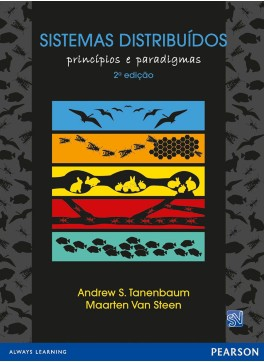
\includegraphics[width=\textwidth]{capa-livro}
    \end{column}
    \begin{column}{0.75\textwidth}
      \begin{block}{Sistemas Distribuídos: Princípios e Paradigmas, 2ª edição (em português) ou 3ª edição (em inglês, gratuita)}
        Autores: Andrew S. Tanenbaum e Maarten van Steen\\
        Pearson Prentice Hall
      \end{block}
      \begin{block}{Slides}
        Exceto se indicado o contrário, os slides serão baseados nos slides do prof. Maarten van Steen.
      \end{block}
    \end{column}
  \end{columns}
\end{frame}


\begin{frame}
  \frametitle{Sistemas Distribuídos: definição}

  Um sistema distribuído é um sistema de software que garante:

  \begin{quote}
    uma coleção de \alert{elementos de computação autônomos} que são vistos pelos usuários como um \alert{sistema único e coerente}
  \end{quote}

  \begin{block}{Características importantes}
    \begin{itemize}
    \item Elementos de computação autônomos, também denominados \emph{nós} (ou \emph{nodos}), sejam eles dispositivos de hardware ou processos de software
    \item Sistema único e coerente: usuários ou aplicações veem um único sistema $\Rightarrow$ nós precisam \alert{colaborar} entre si
    \end{itemize}
  \end{block}

\end{frame}

\begin{frame}
  \frametitle{Coleção de nós autônomos}
  \begin{block}{Comportamento independente}
    Cada nó é autônomo e, portanto, \alert{tem sua própria percepção de tempo}: não há um \alert{relógio global}. Leva a problemas fundamentais de sincronização e de coordenação.
  \end{block}

  \begin{block}{Coleção de nós}
    \begin{itemize}
    \item Como gerenciar \emph{associações em grupos}
    \item Como saber se você realmente está se comunicando com um \emph{(não-)membro autorizado do grupo}
    \end{itemize}
  \end{block}
\end{frame}

\begin{frame}
  \frametitle{Organização}
  \begin{block}{Redes de overlay}
    Cada nós na coleção se comunica apenas com nós no sistema, seus \alert{vizinhos}. O conjunto de vizinhos pode ser dinâmico, ou pode ser descoberto de forma implícita (ex: pode ser necessário procurá-lo)
  \end{block}

  \begin{block}{Tipos de overlay}
    Um exemplo bem conhecido de redes de overlay: \emph{sistemas peer-to-peer}
    \begin{description}
    \item[Estruturada] cada nó tem um \emph{conjunto bem definido de vizinhos} com os quais pode comunicar (árvore, anel)
    \item[Não estruturada] cada nó tem referências a \emph{um conjunto aleatoriamente selecionado de outros nós} do sistema
    \end{description}
  \end{block}
\end{frame}

\begin{frame}
  \frametitle{Sistema coerente}
  \begin{block}{Essência}
    A coleção de nós opera sempre da mesma forma, não importando onde, quando ou como a interação entre um usuário e o sistema acontece
  \end{block}

  \begin{exampleblock}{Exemplos}
    \begin{itemize}
    \item Um usuário não consegue dizer onde a computação está acontecendo
    \item Onde especificamente os dados estão armazenados deveria ser irrelevante para a aplicação
    \item O dado ser ou não replicado deveria estar completamente escondido
    \end{itemize}
  \end{exampleblock}

  A palavra chave é \alert{transparência de distribuição}
\end{frame}

\setintersectionbg

\begin{frame}[standout]
  \textbf{O problema: falhas parciais}

  É inevitável que a qualquer momento um \alert{pedaço} do sistema
  distribuído falhe. Esconder essas falhas parciais e sua recuperação
  normalmente é muito difícil (em geral, é impossível)
\end{frame}

\setsectionbg

\begin{frame}{Middleware: o SO dos sistemas distribuídos}

  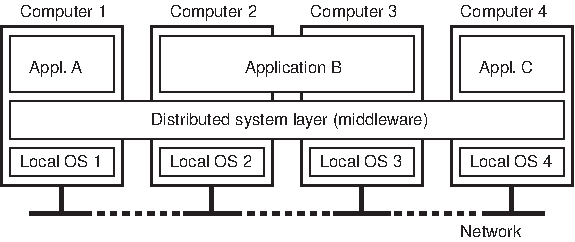
\includegraphics{01-01}

  \begin{block}{O que tem em um middleware?}
    Grosso modo, um conjunto de funções e componentes que não precisam ser reimplementados por cada aplicação separadamente.
  \end{block}

\end{frame}

\begin{frame}{Objetivos de sistemas distribuídos:}

  \begin{itemize}

  \item Disponibilização de recursos compartilhados
  \item Transparência de distribuição
  \item Abertura
  \item Escalabilidade

  \end{itemize}

\end{frame}

\begin{frame}
  \frametitle{Compartilhamento de recursos}
  \begin{exampleblock}{Exemplos clássicos}
    \begin{itemize}
    \item Compartilhamento de dados e arquivos na nuvem
    \item \textit{Streaming} multimídia \textit{peer-to-peer}
    \item Serviços de mensagens compartilhadas
    \item Serviços de hospedagem web compartilhados (à lá redes de distribuição de conteúdo)
    \end{itemize}
  \end{exampleblock}

  \begin{block}{A ponto de pensarmos que:}
  \begin{quotation}
    ``A rede é o computador''
    \begin{flushright}
      \small John Gage, à época na Sun Microsystems
    \end{flushright}
  \end{quotation}
\end{block}
\end{frame}

\begin{frame}{Transparência de distribuição}
  % \vspace*{-0.25cm}
  Tipos:
  \small
  \begin{center}
    \renewcommand{\arraystretch}{1.2}
    {\footnotesize\sffamily
      \begin{tabular}{|l|b{8cm}|} \hline
        \alert{Transparência} & \alert{Descrição} \\ \hline\hline
        Acesso &
            Esconder diferenças entre as representações de dados e mecanismos de invocação \\
	    \hline
        Localização &
	    Esconder onde o objeto está localizado \\
	    \hline
        Relocalização &
            Esconder que um objeto pode ser movido para outra localidade \emph{enquanto está sendo utilizado} \\
	    \hline
        Migração &
            Esconder que um objeto pode ser movido para outra localidade \\
	    \hline
        Replicação &
	    Esconder que um objeto está sendo replicado \\
	    \hline
        Concorrência &
            Esconder que um objeto pode ser compartilhado entre diferentes usuários independentes \\
	    \hline
        Falhas &
            Esconder falhas e a possível recuperação de um objeto \\
	    \hline
    \end{tabular}}
  \end{center}
  \onslide<2->
  \begin{alertblock}{Nota}
    Transparência de distribuição é um objetivo nobre, mas atingi-lo são outros quinhentos...
  \end{alertblock}

\end{frame}

\begin{frame}{Graus de transparência}
  \small
  \begin{block}{Observação:}
    Tentar fazer com que a distribuição seja totalmente transparente pode ser um exagero:
    \begin{itemize}

    \item<2-> Usuários podem estar localizados em \alert{continentes diferentes}

    \item<3-> \alert{Esconder completamente as falhas} da rede e dos nós é  (teoricamente e na prática) \textbf{impossível}

      \begin{itemize}

      \item Você não consegue distinguir um computador lento de um que está falhando
      \item Você nunca consegue ter certeza de que um servidor terminou de realizar uma operação antes dele ter falhar

      \end{itemize}

    \item<4-> Transparência completa terá um \alert{custo no desempenho}, que irá expor a distribuição do sistema

      \begin{itemize}

      \item Manter caches web \emph{rigorosamente} atualizados com o original
      \item Realizar \textit{flush} das operações de escrita para garantir tolerância a falhas

      \end{itemize}

    \end{itemize}
  \end{block}
\end{frame}

\begin{frame}{Abertura de sistemas distribuídos}

  \begin{block}{Sistemas distribuídos abertos}
    São capazes de interagir com outros sistemas abertos:

    \begin{itemize}
    \item devem respeitar \alert{interfaces} bem definidas
    \item devem ser facilmente \alert{interoperáveis}
    \item devem permitir a \alert{portabilidade} de aplicações
    \item devem ser fáceis de \alert{estender}
    \end{itemize}
  \end{block}

  \onslide<2->
  \begin{block}{A abertura dos sistemas distribuídos os tornam independentes de:}
    \begin{itemize}
    \item hardware
    \item plataformas
    \item linguagens
    \end{itemize}
  \end{block}

\end{frame}

\begin{frame}
  \frametitle{Políticas versus Mecanismos}

  \begin{block}{A implementação de abertura requer diferentes \alert{políticas}}
    \begin{itemize}
    \item Qual o nível de consistência necessária para os dados no cache do cliente?
    \item Quais operações podem ser realizadas por programas que acabamos de baixar da Internet?
    \item Quais os requisitos de QoS podem ser ajustados face a variações na banda disponível?
    \item Qual o nível de sigilo necessário para a comunicação?
    \end{itemize}
  \end{block}

  \onslide<2->
  \begin{block}{Idealmente, sistemas distribuídos proveem apenas \alert{mecanismos}:}
    \begin{itemize}
    \item Permitem a atribuição de políticas (dinâmicas) de cache
    \item Possuem diferentes níveis de confiança para código externo
    \item Proveem parâmetros de QoS ajustáveis por fluxo de dados
    \item Oferecem diferentes algoritmos de criptografia
    \end{itemize}
  \end{block}

\end{frame}

\begin{frame}
  \frametitle{Políticas versus Mecanismos}
  \begin{block}{Observação}
    Quanto mais estrita for a separação entre políticas e mecanismos, mais nós precisamos garantir o uso de mecanismos apropriados, resultando potencialmente em muitos parâmetros de configuração e um gerenciamento mais complexo
  \end{block}
  \begin{block}{Como encontrar um equilíbrio?}
    Definir políticas estritas normalmente simplifica o gerenciamento e reduz a complexidade, por outro lado isso implica em menos flexibilidade. Não há uma solução simples.
  \end{block}
\end{frame}

\begin{frame}
  \frametitle{Escalabilidade em Sistemas Distribuídos}

  \begin{block}{Observação:}
    Muitos desenvolvedores de sistemas distribuídos modernos usam o adjetivo ``escalável'' sem deixar claro o \alert{porquê} deles escalarem.
  \end{block}

  \pause

  \begin{block}{Escalabilidade se refere a pelo menos três componentes:}
    \begin{itemize}
    \item Número de usuários e/ou processos -- \alert{escalabilidade de tamanho}
    \item Distância máxima entre nós -- \alert{escalabilidade geográfica}
    \item Número de domínios administrativos -- \alert{escalabilidade administrativa}
    \end{itemize}
  \end{block}

  \pause

  \begin{alertblock}{Observação:}
    A maior parte dos sistemas escalam apenas (e até certo ponto) em
    tamanho. A solução(?!): servidores potentes. Hoje em dia, o
    desafio é conseguir escalabilidade geográfica e administrativa.
  \end{alertblock}

\end{frame}

\begin{frame}
  \frametitle{Dificuldade para obtenção de escalabilidade}
  Um sistema completamente descentralizado tem as seguintes características:

  \begin{itemize}
  \item Nenhuma máquina tem informação completa sobre o estado do sistema
  \item Máquinas tomam decisões baseadas apenas em informação local
  \item Falhas em uma máquina não devem arruinar a execução do algoritmo
  \item Não é possível assumir a existência de um relógio global
  \end{itemize}
\end{frame}

\begin{frame}
  \frametitle{Técnicas de escalabilidade}

  Ideia geral: esconder latência de comunicação

  \begin{block}{Não fique esperando por respostas; faça outra coisa}
    \begin{itemize}
    \item Utilize \alert{comunicação assíncrona}
    \item Mantenha diferentes \textit{handlers} para tratamento de mensagens recebidas
    \item \alert{Problema:} nem toda aplicação se encaixa nesse modelo
    \end{itemize}
  \end{block}

\end{frame}

\begin{frame}
  \frametitle{Técnicas de escalabilidade}

  \begin{block}{Particionamento de dados e computação em muitas máquinas}
    \begin{itemize}
    \item Mova a computação para os clientes (ex: Javascript, Applets Java, etc.)
    \item Serviços de nomes decentralizados (DNS)
    \item Sistemas de informação decentralizados (WWW)
    \end{itemize}
  \end{block}

\end{frame}

\begin{frame}
  \frametitle{Técnicas de escalabilidade}

  \begin{block}{Replicação/caching}
    Faça cópias dos dados e disponibilize-as em diferentes máquinas:

    \begin{itemize}
    \item Bancos de dados e sistemas de arquivos replicados
    \item Sites web ``espelhados''
    \item Caches web (nos navegadores e nos \textit{proxies})
    \item Cache de arquivos (no servidor e nos clientes)
    \end{itemize}
  \end{block}

\end{frame}

\begin{frame}
  \frametitle{Escalabilidade -- O Problema}
  \begin{block}{Observação}
    Aplicar técnicas para obtenção de escalabilidade é fácil, exceto por uma problema:

    \begin{itemize}
    \item<2-> Manter múltiplas cópias (em cache ou replicadas) leva a \alert{inconsistências}: a modificação em uma cópia a torna diferente das demais
    \item<3-> Manter as cópias consistentes requer \alert{sincronização global} em cada modificação
    \item<4-> Sincronização global impossibilita soluções escaláveis
    \end{itemize}
  \end{block}

  \begin{block}{Observação:}<5->
    Se nós pudermos tolerar inconsistências, nós podemos reduzir a
    dependência em sincronização globais, mas \alert{tolerar
      inconsistências é algo que depende da aplicação}.
  \end{block}

\end{frame}


\begin{frame}
  \frametitle{Armadilhas no desenvolvimento de sistemas distribuídos}
  \begin{block}{Observação:}
    Muitos sistemas distribuídos se tornam desnecessariamente complexos por causa de ``consertos'' ao longo do tempo. Em geral, há muitas \alert{hipóteses falsas}:

    \begin{itemize}
    \item<2-> A rede é confiável
    \item<3-> A rede é segura
    \item<4-> A rede é homogênea
    \item<5-> A topologia da rede não muda
    \item<6-> A latência é zero
    \item<7-> Largura de banda é infinita
    \item<8-> O custo de transporte é zero
    \item<9-> A rede possui um administrador
    \end{itemize}
  \end{block}
\end{frame}

\end{document}
